%--------------------------------------------------------------------------------------------------
% 
\chapter{Retrieval Augmented Approach}
\label{ch:retrieval}

%In the next chapter,\todo{you mean this chapter (4)? or the next one (5)? Would be simpler and less ambiguous to say, "This chapter outlines our proposed method [\ldots]"} we will outline our proposed method, which uses an information retrieval (IR) approach to a large-scale multi-label classification problem to address the challenges of multilinguality, rare languages, low-resource environments, long-tailed label distributions, text truncation, and frequent label changes.

%We will start by introducing the selected baseline model and comparing it against baselines of models fine-tuned on a well-known and comparable $EURLEX57K$ dataset presented in Chapter~\ref{ch:data}. 
%This will be followed by discussing the embedding models we plan to employ. 
%Finally, we will present and discuss our proposed method and share preliminary zero-shot results.

In this chapter, we will first outline our proposed method, which uses an information retrieval (IR) approach to a large-scale multi-label classification problem.
This will be followed by a discussion of the embedding models we plan to employ. 
We will continue by introducing the selected baseline model and comparing it against baselines of models fine-tuned on a well-known and comparable $EURLEX57K$ dataset presented in Chapter~\ref{ch:data}. 
Finally, we will present and discuss zero-shot experiments and share preliminary results.

\section{Introduction}

In contrast to most models in XMTC and MLTC, which use end-to-end neural network training, our approach handles the classification and information retrieval tasks separately.
With this approach, we aim to address the challenges of multilinguality, rare languages, low-resource environments, long-tailed label distributions, text truncation, and frequent label changes.
%  in this initial research phase

\begin{figure}[h!]
  \centering
  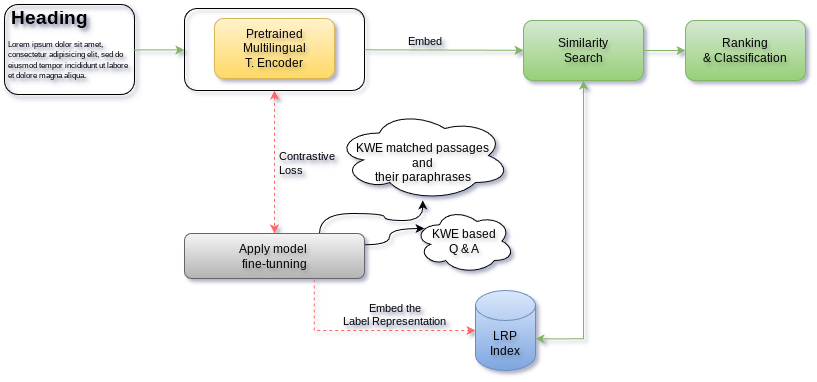
\includegraphics[width=1\textwidth]{figures/newsmon_model.png}
  \caption{The proposed framework: After model fine-tuning, we store label-relevant passages (LRP) together with label information in the LRP index (red line). 
  At inference time (green line), we search for similar passages, rank the search results, extract the label information and classify.}
  \label{fig:newsmon_model}
\end{figure}

We propose a straightforward approach that utilizes the pre-trained embedding IR model to encode both documents and label-relevant text passages (LRP).
During inference, the document is embedded as a query using the encoder and the LRP index is searched to retrieve all relevant labels.
For the classification task, we use the ranked top N similarity search results from the encoded LRP index based on an LRP-calibrated similarity threshold. 
To build an LRP index, we map each label with every encoded LRP for a particular label.
From the LRP, corresponding labels are mapped, and the IR ranking score is interpreted as classification probability, where only the highest score for each duplicate label match is considered~\ref{fig:newsmon_model}.
We opted to evaluate our method using a zero-shot approach for initial testing, meaning we did not fine-tune the IR model for the preliminary research.
For the zero-shot approach, we carry out similarity threshold calibration on the validation set to determine a per-label and overall average global similarity threshold, at which point classification for a given label becomes positive. 

We used re-matched text spans (MTS) on the $NewsMon$ dataset to identify text locations corresponding to specific labels for encoding LRP representations. 
We extracted different text context sizes based on sentence segmentation to form an LRP.
This extracted dataset will be our foundation for the model fine-tuning, which requires positive and negative query-passage pairs.
The best performance is achieved if the negative instances are similar but lack the target label—hard negatives (HN).
For mining the HN instances (those that are similar but lack the target label) from our dataset, we can use either a non-fine-tuned model, a competitive model~\parencite{wang2024multilinguale5textembeddings, xiao2024cpackpackagedresourcesadvance}, or the BM25 search algorithm.

\section{The Embedding Model}
For the document and LRP embeddings, we focused particularly on the M3-Embedding model (BGE-M3), noted for its adaptability across Multi-Linguality, Multi-Functionality, and Multi-Granularity~\parencite{chen2024bgem3embeddingmultilingualmultifunctionality}. 
The BGE-M3 model supports the semantic retrieval of over 100 operational languages. 
Additionally, it can simultaneously perform the three prevalent retrieval functionalities: dense retrieval, multi-vector retrieval, and sparse retrieval. 
Moreover, it can process inputs of varying lengths, ranging from sentences to documents containing as many as 8,192 tokens.
Considering its size and multilingual capabilities, the model achieves state-of-the-art performance on the MTEB~\parencite{muennighoff2022mteb} and Miracl~\parencite{zhang2023miracl} information retrieval benchmarks.

BGE-M3 is trained in two stages.
First, the XLM-RoBERTa model modified by the RetroMAE~\parencite{xiao2022retromae} is pre-trained using extensive unsupervised data, where only dense retrieval undergoes training using a basic form of contrastive learning. 
In the second stage, self-knowledge distillation is employed, fine-tuning the embedding model to refine the three retrieval functionalities.
Namely, it computes a weighted combined Noise-Contrastive Estimation loss (InfoNCE), introduced by \textcite{oord2019representationlearningcontrastivepredictive}, for each of the three functionalities.
Given that the $NewsMon$ dataset contains numerous named entities, the sparse retrieval, which compares token similarities between an encoded query and a text passage, can benefit our task.

\section{The Baseline Experiments}

To evaluate our method, we fine-tuned the multilingual pre-trained language model (PLM) and used it as a baseline classifier.
Namely, we selected XLM-RoBERTa-base~\parencite{conneau2019xlmr} from Huggingface~\parencite{wolf-etal-2020-transformers} and fine-tuned it on a $NewsMon_{sl+cls}$ using a Binary cross-entropy loss. 
Our previous research observed that the XLM-RoBERTa-base (XLM-R) model consistently outperforms the multilingual BERT~\parencite{ivacic2024comparing}. 
This is also the model from which the targeted embedding models were initially derived~\parencite{chen2024bgem3embeddingmultilingualmultifunctionality, wang2024multilinguale5textembeddings}.

We eliminated labels that appear only once to fine-tune the baseline model and conducted uniform random sampling to divide the $NewsMon_{sl+cls}$ dataset into an 80/10/10 split for the train, validation, and test sets, respectively. 
The labels in the $NewsMon_{sl+cls}$ dataset occur only once because of the removal of OCR, transcripts, and other non-publicly available data, as well as because the data was sampled only for selected labels and for a limited period.

For the baseline model training, we did not perform hyper-parameter optimisation; all the models are fine-tuned using the default set of hyper-parameters in the Transformers library, optimised for a large selection of common NLP tasks.
More precisely, following the methodology of \textcite{park2022efficient, chalkidis-etal-2019-large} we used similar settings as for $EURLEX57K$ dataset:
\begin{itemize}\itemsep=0pt
  \item AdamW optimiser with a learning rate of $3e-05$.
  \item Weight decay set to 0.01 for regularisation.
  \item Training for a maximum of 30 epochs.
  \item Batch size of 16.
  \item Dropout rate of 0.1.
  \item Maximum length of 512 sub-word tokens.
  \item Best model selection based on the validation set micro F1-score.
\end{itemize}
Based on initial test runs, we increased the maximum number of epochs from 20 to 30. 
We observed that learning stopped improving near the epoch 30.
Additionally, we increased the batch size to 16 to speed up training.
We repeated the fine-tuning process five times, setting a different random seed and re-shuffling the training set.

To evaluate the performance and, more importantly, to verify the implementation of our baseline classifier, we also fine-tuned the same PLM with the $EURLEX57K$ dataset.
All previous research reported evaluation metrics on the $EURLEX57K$ dataset model fine-tuned on a monolingual BERT; therefore, we couldn't compare directly with reported results.
%\todo{somewhere in this section, maybe worth saying that the "baseline" is more computationally expensive (I guess?) and involves more annotated data than your proposed approach}
% TODO: check this ... media outlet rules might influence rare label frequency.

To assess the feasibility of our approach with the selected BGE-M3 model, we conducted an additional zero-shot baseline experiment using the simplest method possible. 
For this experiment, we first embedded the training set and stored these embeddings in an index, along with their corresponding labels. 
Next, we chose samples from the test set, using their labels as ground truth for the classification task. 
Finally, we performed a cosine similarity search for each test sample and assigned labels from the closest training instance as predictions. 
We did not fine-tune the model, utilize label-relevant passages, or implement any ranking system.
Additionally, we didn't search at which threshold the similarity search yields the best classification results.

\clearpage 

\begin{table}[h]
    \centering
    \resizebox{\textwidth}{!}{%
        \begin{tabular}{lccccccc}
        \hline
        \textbf{Model} & \textbf{Corpus} & \textbf{Micro F1} & \textbf{Micro P} & \textbf{Micro R} & k & \textbf{R-Precision@k} & \textbf{NDCG@k} \\
        \hline
        BERT & $EURLEX57K$ & \textbf{73.2}  & - & - & 5 & \textbf{79.6} & \textbf{82.3}  \\
        XLM-R & $EURLEX57K$ & 68.765 $\pm$ 0.182 & 85.086 $\pm$ 0.318 & 57.698 $\pm$ 0.246 & 5 & 76.256 $\pm$ 0.218 & 79.200 $\pm$ 0.193 \\
        \hline
        XLM-R & $NewsMon_{sl+cls}$ & 61.559 $\pm$ 2.306 & \textbf{85.952} $\pm$ 0.408 & 47.988 $\pm$ 2.710 & 3 & 79.649 $\pm$ 1.740 & 80.084 $\pm$ 1.819 \\
        BGE-M3 & $NewsMon_{sl+cls}$ & \textbf{66.151} & 65.259 & \textbf{67.067} & - & - & - \\
        \hline
        \end{tabular}
    }
    \caption{Baseline XLM-R classifier performance metrics for $EURLEX57K$ and $NewsMon_{sl+cls}$ corpora. For BERT PLM, we show metrics reported by \textcite{chalkidis-etal-2019-large}; for the XLM-R model, we show our baseline classifier metrics. We report at K = corpus label cardinality~\parencite{chalkidis-etal-2019-large}.}
\label{tab:baseline_metrics}
\end{table}

The evaluation results of the baseline classifier on the test set are presented in Table~\ref{tab:baseline_metrics}.
If we first compare conventional PLM models, we can see that the performance dropped noticeably when using a multilingual model for $EURLEX57K$ text. 
Observing the standard deviation with micro-averaged F1 and recall, we can see that training the baseline classifier on a $EURLEX57K$ dataset has much more predictive results compared to $NewsMon_{sl+cls}$. 
$NewsMon_{sl+cls}$ fine-tuned baseline classifier has a significantly worse recall, indicating that the model struggles to identify all the relevant labels for each instance. 
Since the precision of the two models is close, we can assume that the $NewsMon_{sl+cls}$ model has a higher rate of false negatives compared to the $EURLEX57K$ model.

Next, comparing a simple similarity search with conventional PLM, we can observe that similarity search combined with BGE-M3 embeddings outperforms the XLM-R baseline classifier on micro F1 score by improving overall recall.
Consequently, we can view the XLM-R model as being more precise but considerably more conservative, favouring false negatives over false positives. 

We noticed duplication phenomena in the dataset when we analysed the individual classification samples for the zero-shot experiment.
Some news articles were duplicated but appeared in different outlets or news aggregators. 
Some were very similar in content, for instance, a summary of the official press release or social media posts with picture changes that are not reflected in the content itself (see Table~\ref{tab:social_dup}).
We believe this is a significant factor in the performance of the simple similarity search. 
Further analysis would be necessary to confirm this.


\begin{table}[h]
    \centering
    \resizebox{\textwidth}{!}{%
        \begin{tabular}{l}
        \hline
        \makecell{
        [IMAGE]: River Krka in Novo mesto, S... \\
\\
River Krka in Novo mesto, Slovenia \#visitdolenjska \#igdolenjska \#visitslovenia \#ifeelslovenia \#geoslovenija \#nasvetzaizlet \\ 
\#kampadanes \#ig\_brilliant \#special\_shots \#main\_vision \#discoverglobe \#ourplanetdaily \#earthofficial \#earthoutdoors \\ 
\#splendid\_view \#roamtheplanet \#stunning\_shots \#amazing\_shots \#theglobewanderer \#wanderlust \#travelphotography \\ 
\#travelgram \#traveladdict \#worldbestgram \#ig\_captures \#djimini3pro \#ig\_exyu \#beautifuldestinations \#nature \#naturephotograph
} \\
        \hline
        \end{tabular}
    }
    \caption{An example social media post from $NewsMon_{sl+cls}$ corpora which is repeated for every update.}
\label{tab:social_dup}
\end{table}
